%
% rechteck.tex
%
% (c) 2021 Prof Dr Andreas Müller, OST Ostschweizer Fachhochschule
%
\section{Rechteckige Membran
\label{buch:pde:section:rechteck}}
\rhead{Rechteckige Membran}
Als Beispiel für die Lösung des in
Abschnitt~\ref{buch:pde:subsection:eigenwertproblem}
aus der Wellengleichung abgeleiteten Eigenwertproblems
mit Hilfe von Separation betrachten wir ein rechteckiges Gebiet.

\subsection{Differentialgleichung und Randbedingungen}
Wir betrachten das Gebiet
\[
G
=
(0,a) \times (0,b) 
=
\{ (x,y) \mid 0< x <a\wedge 0<y<b\}.
\]
Gesucht ist eine Lösung des Eigenwertproblems
\begin{equation}
\Delta U = -\lambda^2 U
\label{buch:pde:rechteck:eqn:dgl}
\end{equation}
auf $G$ mit den homogenen Randbedingungen
\[
\left.
\begin{aligned}
U(0,y) &= 0\\
U(a,y) &= 0
\end{aligned}
\;
\right\}
\forall y \in (0,b)
\qquad
\text{und}
\qquad
\left.
\begin{aligned}
U(x,0) &= 0\\
U(x,b) &= 0
\end{aligned}
\;
\right\}
\forall x \in (0,a).
\]
Dieses Gebiet lässt sich bestens in kartesischen Koordinaten
beschreiben, so dass wir auch den Laplace-Operator in den
gleichen Koordinaten ansetzen können.
Wir verwenden also im folgenden
\[
\Delta = \frac{\partial^2}{\partial x^2} + \frac{\partial^2}{\partial y^2}.
\]


\subsection{Separation}
Wir setzen die Lösung als Produkt von Funktionen, die nur von einer
der Variablen abhängen, nämlich
\[
U(x,y)
=
X(x) \cdot Y(y).
\]
Durch Einsetzen in die
Differentialgleichung~\eqref{buch:pde:rechteck:eqn:dgl}
erhalten wir
\[
X''(x) \cdot Y(y) + X(x)\cdot Y''(y) = -\lambda^2 X(x)\cdot Y(y).
\]
Nach Division durch $X(x)\cdot Y(y)$ können wir separieren in 
\[
\frac{X''(x)}{X(x)}=-\lambda^2 - \frac{Y''(y)}{Y(y)}.
\]
Da wir Schwingungslösungen erwarten, schreiben wir die Lösungen
in der Form $-\mu^2$. 
So erhalten wir die beiden Differentialgleichungen
\[
\begin{aligned}
X''(x) &= -\mu^2 X(x)&&x\in (0,a)
\\
Y''(y) &= (-\lambda^2-\mu^2) Y(y)&& y\in(0,b)
\end{aligned}
\]

Die Funktionen $X(x)$ und $Y(y)$ müssen homogene Randbedingungen
erfüllen, also
\[
\begin{aligned}
X(0) &= 0\\
X(a) &= 0
\end{aligned}
\qquad\text{und}\qquad
\begin{aligned}
Y(0) &= 0\\
Y(b) &= 0
\end{aligned}
\]

\subsection{Lösung der Differentialgleichungen}
Die allgemeine Lösung der Differentialgleichung $X''(x) = -\mu^2 X(x)$
ist eine Funktion der Form
\[
X(x) = A\cos\mu x + B\sin\mu x.
\]
Die Randbedingung für $x=0$ ist
\[
X(0) = A = 0
\]
bedeutet, dass nur der Sinus-Term verwendet werden muss.
Die Randbedingung am rechten Rand wird dann
\[
X(a) = B\sin\mu a.
\]
Da $B$ nicht auch verschwinden kann, muss $\sin\mu a=0$ sein.
Die Nullstellen der Sinus-Funktion sind alle ganzzahligen Vielfachen
\[
\mu a = k\pi,\qquad k\in\mathbb{Z}
\Rightarrow
\mu = \frac{k\pi}{a}\qquad k\in\mathbb{Z}.
\]
Die negativen $k$ geben die gleichen Lösungsfunktionen wie die positiven
$k$, man kann sich daher auf die positiven $k$ beschränken.
Die Lösungen sind daher
\[
X_k(x) = \sin \frac{k\pi}{a}x.
\]

Für die Gleichung $Y''(y)=(-\lambda^2 +\mu^2)Y(y)$ folgt auf ganz analoge
Weise, dass ihre Lösungen die Form
\[
Y_l(y)
=
\sin \frac{k\pi}{b}y.
\]

Aus $X_k(x)$ und $Y_l(y)$ können jetzt die Lösungen
\begin{equation}
U_{kl}(x,y) = \sin \frac{k\pi}{a} x\cdot \sin\frac{k\pi}{b}y
\label{buch:pde:rechteck:eqn:ukl}
\end{equation}
zusammengesetzt werden, die homogene Randbedingungen entlang
des ganzen Randes des Rechtecks erfüllen.

Die Funktionen $X_k(x)$ hat weitere Nullstellen für $x$-Werte, für
die $k\pi x/a$ ein ganzzahliges Vielfaches von $k$ ist, also  wenn
\[
\frac{kx}{a}
=
\frac{x}{a/k}
\]
eine ganze Zahl ist.
Dies tritt ein, wenn $x$ ein ganzzahliges Vielfaches von $a/k$ ist.
Ebenso hat die Funktion $Y_l(y)$ Nullstellen, wenn $y$ ein ganzzahliges
Vielfaches von $b/l$ ist.
Die Funktion $U_{kl}(x,y)$ verschwindet daher auf allen Geraden
parallel zur $y$-Achse an $x$-Koordinaten, die Vielfache von $a/k$ sind
und auf allen Geraden parallel zur $x$-Achse an $y$-Koordinaten, die
Vielfache von $b/l$ sind.

\subsection{Eigenfrequenzen}
\begin{figure}
\centering
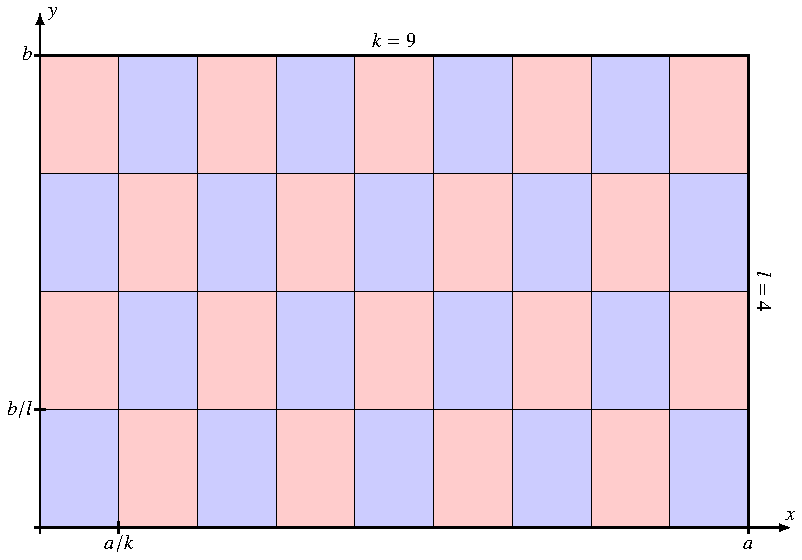
\includegraphics{chapters/090-pde/images/rechteck.pdf}
\caption{Vorzeichen und Knotenlinie der Eigenfunktion
$U_{kl}(x,y)$ des Laplace-Operators auf dem Rechteck $(0,a)\times (0,b)$.
In den blauen Rechtecken gilt $U_{kl}(x,y)>0$ in den roten gilt
$U_{kl}(x,y)<0$.
die vertikalen und horizontalen schwarzen Linien sind Knotenlinien
der Eigenfunktion, ihre $x$-Koordinaten sind Vielfache von $a/k$,
die $y$-Koordinaten sind Vielfache von $b/l$.
\label{buch:pde:rechteck:fig:knoten}}
\end{figure}
Die Lösungen $U_{kl}(x,y)$ aus \eqref{buch:pde:rechteck:eqn:ukl}
sind Lösungen der ursprünglichen Differentialgleichung 
$\Delta U=-\lambda^2 U$.
Durch Einsetzen lassen sich jetzt auch die Eigenwerte bestimmen:
\begin{align*}
\Delta U_{kl}(x,y)
&=
-\frac{k^2\pi^2}{a^2} \sin\frac{k\pi}{a}x\cdot \sin\frac{k\pi}{b}y
-\frac{l^2\pi^2}{b^2} \sin\frac{k\pi}{a}x\cdot \sin\frac{k\pi}{b}y
=
-\biggl(\frac{k^2\pi^2}{a^2}+\frac{l^2\pi^2}{b^2}\biggr) U_{kl}(x,y)
\end{align*}
Die Eigenfrequenzen einer rechtecking schwingenden Membran sind also
\[
\lambda
=
\sqrt{
\frac{k^2\pi^2}{a^2}+\frac{l^2\pi^2}{b^2}
}.
\]
Die Vorzeichen und die Knotenlinien der $U_{kl}(x,y)$ des
Eigenwertproblems ist in Abbildung~\ref{buch:pde:rechteck:fig:knoten}
dargestellt.
